\documentclass[11pt]{article}

\usepackage[utf8]{inputenc}
\usepackage{amsmath}
\usepackage{li		stings}
\usepackage{amsfonts}
\usepackage{amssymb}
\usepackage{color}
\usepackage{inputenc}
\usepackage{graphicx}

\usepackage[left=1.2in,top=1.2in,right=1.2in,bottom=1.0in]{geometry} % Document margins

\title{\textbf{Operating System Lab Project \\ 
	Theme B, Group 12 \\
    Virtual Memory for the Geek OS \\
    Final report
	 }}

\definecolor{mygreen}{rgb}{0,0.6,0}
\definecolor{mygray}{rgb}{0.5,0.5,0.5}
\definecolor{mymauve}{rgb}{0.58,0,0.82}

\author{Rohit Kumar \\ 120050028 \\ rohit@cse.iitb.ac.in
		\and 
		Deependra Patel \\ 120050032 \\ deependra@cse.iitb.ac.in
		\and
		Jayesh Bageriya \\ 120050022 \\ jayeshbageriya@cse.iitb.ac.in
        \\
		\and 
		Abhishek Thakur \\ 120050008 \\ abhishekthakur@cse.iitb.ac.in
		}

\date{\today}

\lstset{ %
  backgroundcolor=\color{white},   % choose the background color; you must add \usepackage{color} or \usepackage{xcolor}
  basicstyle=\footnotesize,        % the size of the fonts that are used for the code
  breakatwhitespace=false,         % sets if automatic breaks should only happen at whitespace
  breaklines=true,                 % sets automatic line breaking
  captionpos=b,                    % sets the caption-position to bottom
  commentstyle=\color{mygreen},    % comment style
  escapeinside={\%*}{*)},          % if you want to add LaTeX within your code
  extendedchars=true,              % lets you use non-ASCII characters; for 8-bits encodings only, does not work with UTF-8
  frame=single,                    % adds a frame around the code
  keepspaces=true,                 % keeps spaces in text, useful for keeping indentation of code (possibly needs columns=flexible)
  keywordstyle=\color{red},       % keyword style
  language=vhdl,                 % the language of the code
  numbers=left,                    % where to put the line-numbers; possible values are (none, left, right)
  numbersep=5pt,                   % how far the line-numbers are from the code
  numberstyle=\tiny\color{mygray}, % the style that is used for the line-numbers
  rulecolor=\color{black},         % if not set, the frame-color may be changed on line-breaks within not-black text (e.g. comments (green here))
  showspaces=false,                % show spaces everywhere adding particular underscores; it overrides 'showstringspaces'
  showstringspaces=false,          % underline spaces within strings only
  showtabs=false,                  % show tabs within strings adding particular underscores
  stepnumber=2,                    % the step between two line-numbers. If it's 1, each line will be numbered
  stringstyle=\color{mymauve},     % string literal style
  tabsize=2,                       % sets default tabsize to 2 spaces
  title=\lstname                   % show the filename of files included with \lstinputlisting; also try caption instead of title
}

\begin{document}

\maketitle


\begin{abstract}

This projects involves the extension of a tiny operating system called \textbf{GeekOS} for x86 PCs which serve as a simple but realistic example of an OS kernel running on real hardware to use the concept of \textbf{virtual memory} which is a powerful feature of an operating system that provides an illusion to compensate for shortages of physical memory by temporarily transferring pages of data from random access memory (RAM) to disk storage. 

It maps memory addresses used by a program, called virtual addresses, into physical addresses in computer memory. Main storage as seen by a process or task appears as a contiguous address space or collection of contiguous segments. The operating system manages virtual address spaces and the assignment of real memory to virtual memory. Address translation hardware in the CPU, often referred to as a memory management unit or MMU, automatically translates virtual addresses to physical addresses.

The project will talk about the implementation of modules required for this feature and some of the data structures and algorithms which make it efficient \textit{eg.} multilevel page tables, page replacement algorithms, translation look-aside buffers etc. Apart from it consists some special features like pinned pages etc.

\end{abstract}

\pagebreak

\section{Implementation Overview}
\paragraph{}
We have implemented the following features.
\begin{itemize}
\item Multilevel page table
\item Page replacement implementation
\item Loading code in swap space and allocating page frames to processes
\item Non contiguous memory allocation
\item Pinned Pages
\item Swap space allocation
\end{itemize}

Now the next section will talk in detail, providing the higher level and lower level aspects of implementation with the data structures \& algorithms used for it.

\section{Page table (Multilevel)}

When a process requests access to a data in its memory, it is the responsibility of the operating system to map the virtual address provided by the process to the physical address of the actual memory where that data is stored. The page table is where the operating system stores its mappings of virtual addresses to physical addresses, with each mapping also known as a page table entry (PTE).

Every region of the memory that is being accessed should have an entry in the page table.

We have implemented a two level page table with higher level (directory level) indexed on 10 MSB and next level indexed on next 10 bits.


\begin{figure}[ht!]
	\centering
	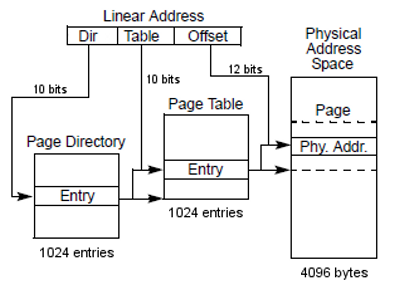
\includegraphics[width=100mm]{p4.png}
	\caption{Two level Page Table}
\end{figure}


Now, the page tables are set. A new page directory is allocated using Alloc\_Page() and then
page tables for the entire region that will be mapped into this memory context are allocated (done in the for loop in below code). Appropriate fields in the page tables and page directories, (represented by the pde\_t and pde\_t data-types) are filled.


\begin{lstlisting}[language=c]

/*
 * Page directory entry datatype.
 * If marked as present, it specifies the physical address
 * and permissions of a page table.
 */
typedef struct {
    uint_t present:1;
    uint_t flags:4;
    uint_t accessed:1;
    uint_t reserved:1;
    uint_t largePages:1;
    uint_t globalPage:1;
    uint_t kernelInfo:3;
    uint_t pageTableBaseAddr:20;
} pde_t;

/*
 * Page table entry datatype.
 * If marked as present, it specifies the physical address
 * and permissions of a page of memory.
 */
typedef struct {
    uint_t present:1;
    uint_t flags:4;
    uint_t accessed:1;
    uint_t dirty:1;
    uint_t pteAttribute:1;
    uint_t globalPage:1;
    uint_t kernelInfo:3;
    uint_t pageBaseAddr:20;
} pte_t;


\end{lstlisting}

\subsection{Kernel Memory Mapping}
\paragraph{}

To set up paging for kernel, we need to allocate a page directory (via Alloc\_Page) and then allocate page tables (also via Alloc\_Page) to cover the entire physical memory. This is done in function Init\_VM in paging.c. The appropriate fields are filled in the page directory entries and page table entries. 

Now, paging is enabled (GeekOS does not use paging by default). This also in function Init\_VM, by calling the routine Enable\_Paging, which is defined in lowlevel.asm. It takes the base address of the page directory as a parameter.

We also need to register a handler for page faults. This is also done in function Init\_VM. Currently, a page fault can occur only when a process attempts to access an invalid address (not present in physical memory). Therefore, we have a handler, Page\_Fault\_Handler in paging.c, which terminates a user program that does this. This handler is registered for the page fault interrupt, interrupt 14, by calling Install\_Interrupt\_Handler.

Now, a call to the Init\_VM function from main.c is called (after Init\_Interrupts).

There will be a single page table for all kernel only threads. The kernel memory should be a one to one mapping of all of the physical memory in the processor. The page table entries for this memory have been marked so that this memory is only accessible from kernel mode.

\subsubsection{Problems Faced}
\paragraph{APIC HOLE}

Some amount of memory is not mapped in kernel VM. Because of this, we got page faults. For solving this problem, we have to separately map this area of memory.
After this fix, processes are being started.



\subsection{User Memory Mapping}
\paragraph{}
There will be a page directory for each user process. The page directory for a user process will contain entries mapping user logical memory to linear memory, but it will also contain entries to address the kernel memory. This is not so that user processes can access kernel memory directly (set the access flags of the kernel memory to prevent them from doing so), but rather so that when an interrupt occurs, the page directory does not need to be changed for the kernel to access its own memory, it will simply use the page directory of the user process that was running when the interrupt occurred. 

The layout of the linear address space of a user process is shown below:


\begin{figure}[ht!]
	\centering
	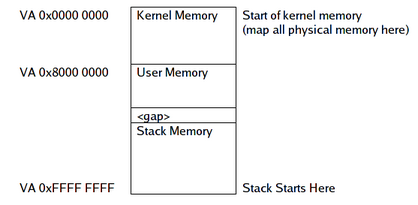
\includegraphics[width=100mm]{vm.png}
	\label{Two level Page Table}
\end{figure}


The next step is to modify the user processes so that the logical addresses they generate are mapped to linear addresses in the user range of memory (i.e., from 0x8000 0000 to 0xFFFF FFFF). This is done in a  new file called uservm.c that will replace userseg.c from previous projects. In the file Makefile.common in the build directory, there is a line which specifies which of userseg.c or uservm.c should be used.

\section{Loading code and allocating frames for user programs}
\paragraph{}

This function takes the buffer containing the executable to load, the no. of bytes in the data, a segment information describing how to load the executable's text and data segments. The working is described as:

\subsection{Load\_User\_Program function}
\begin{itemize}
\item Obtained space requirements for code, data, argument block, and stack
\item Allocated page directory and pages for above and mapped them into user address space (allocating page directory and page tables as needed)
\item Filled in initial stack pointer, argument block address, and code entry point fields in User\_Context
\end{itemize}

\subsection{Copy\_User\_Page}
\paragraph{}
This function fills code and data section of elf file into physical format.

\subsection{Create and destroy user context}
\paragraph{}
Fills the initial stack pointer, argument block address, and code entry point fields in User\_Context. After process is completed, user context is destroyed using Destroy\_user\_context.

After loading the user program the kernel calls the function Switch\_To\_Address\_Space sets the page directory base table and loads the local descriptor table.


\section{Free List Manger}
\paragraph{}
A background kernel thread, which maintains a free list of all the pages (s\_freeList) in physical memory. When a page allocation request is made, it calls the modules for page in, page out. It is already implemented in GeekOS. The modules for page in, page out is done by us.


\section{Swap space}

\paragraph{}
We have used pagefile.bin as a swap file which is initialized to NULL. For every page in the swap space a bit map is kept. 0 bit indicates that the corresponding page is empty (free) in swap space and 1 as filled. The function Find\_space\_on\_paging\_file in paging.c yields the first page whose corresponding bit in bitmap is 0 (index of free page). If a page has to be paged out into the swap space, the free page is found as above and then we use the Write\_to\_paging\_file function which uses the Block\_write function of the file.

Similarly in the case when the address requested has been paged out (found from page table entry), then we page in that page from the swap space and free that page in swap space by modifying the bit map.


The paging file consists of a group of consecutive 512 bytes disk blocks. Calling the routine Get Paging Device() (in geekos/vfs.h) will
return a Paging Device() object; this consists of the block device the paging file is on, the start sector
(disk block number), and the number of sectors (disk blocks) in the paging file. Each page will consume
8 consecutive disk blocks. To read/write the paging device, the functions Block Read() and Block
Write() are used.

\begin{lstlisting}

void Write_To_Paging_File(void *paddr, ulong_t vaddr, int pagefileIndex) {

    KASSERT(0);
    struct Page *page = Get_Page((ulong_t) paddr);
    KASSERT(!(page->flags & PAGE_PAGEABLE)); /* Page must be locked! */
    KASSERT((page->flags & PAGE_LOCKED));
 //Debug("PageFileIndex: 0 <= %d < %d/n", pagefileIndex, bitmapSize);
    if(0 <= pagefileIndex && pagefileIndex < numOfPagingPages){
        int i;
        for(i = 0;i < SECTORS_PER_PAGE; i++){
            Block_Write(pagingDevice->dev, pagefileIndex*SECTORS_PER_PAGE + i + (pagingDevice->startSector),paddr+i*SECTOR_SIZE);      
        }
        Set_Bit(BitmapPaging, pagefileIndex); 
    }
    else {
        Print("In func Write_To_Paging_File: pagefileIndex out of range!");
        KASSERT(0);
        Exit(-1);
    }  
    //struct Page *page = Get_Page((ulong_t) paddr);
    //KASSERT(!(page->flags & PAGE_PAGEABLE));    /* Page must be locked! */
    // TODO_P(PROJECT_VIRTUAL_MEMORY_B, "Write page data to paging file");
}


void Read_From_Paging_File(void *paddr, ulong_t vaddr, int pagefileIndex) {
        KASSERT(0);

    struct Page *page = Get_Page((ulong_t) paddr);
    KASSERT(!(page->flags & PAGE_PAGEABLE));    /* Page must be locked! */

    if(0<=pagefileIndex && pagefileIndex < numOfPagingPages){
        int i;
        for(i = 0;i < SECTORS_PER_PAGE;i++){
            Block_Read(pagingDevice->dev, pagefileIndex*SECTORS_PER_PAGE + i + (pagingDevice->startSector),paddr+i*SECTOR_SIZE);      
        }
    }
    else {
        Print("In func Write_To_Paging_File: pagefileIndex out of range!");
        KASSERT(0);
        Exit(-1);
    }     

    //TODO_P(PROJECT_VIRTUAL_MEMORY_B, "Read page data from paging file");
}

\end{lstlisting}

\section{Page replacement}
\paragraph{}

Implemented in the function \textbf{Find\_Page\_To\_Page\_Out}.

We have implemented the \textbf{one handed clock} page replacement algorithm. A variable/bit \textit{"accessed"} is already present in page table entry which is updated to 1 upon read/write by hardware for that page (already done by GeekOS). 

For, the one handed clock algorithm while hunting a page,
\begin{itemize}
\item  All the physical pages are traversed from the current clock hand (kept as global).
\item If the \textit{accessed} bit is 1 then it is set to 0 while updating the clock hand
\item The first page whose \textit{accessed} bit is 0 is chosen to be swapped out.
\end{itemize}






\section{Pinned Pages}
\paragraph{}
A bool \textbf{pinnedPage} is kept in the page data structure. If it's value is set to 1, then it is locked and cannot be swapped out. Otherwise it is pageable (hence can possibly be swapped out).

The first page frame of every process, i.e. \textbf{page directory} is pinned while other pages are pageable and cannot be swapped out by a page replacement process. Apart from these all pages of kernel are pinned.



\section{Handling Page Faults}
\paragraph{}


For working with paging, the operating system needs to handle page faults. To do this a page fault interrupt handler should be present.

The first thing the page fault handler will need to do is to determine the address of the page fault which can be found out  by calling the Get\_Page\_Fault\_Address() function (present in  geekos/paging.h. Also, the errorCode field of the Interrupt
State data structure passed to the page fault interrupt handler contains information about the faulting
access. This information is defined in the faultcode\_t data type (defined in geekos/paging.h).

\begin{lstlisting}[language=c]
/*
 * Datatype representing the hardware error code
 * pushed onto the stack by the processor on a page fault.
 * The error code is stored in the "errorCode" field
 * of the Interrupt_State struct.
 */
typedef struct {
    uint_t protectionViolation:1;
    uint_t writeFault:1;
    uint_t userModeFault:1;
    uint_t reservedBitFault:1;
    uint_t reserved:28;
} faultcode_t;

\end{lstlisting}



Given a virtual address at which page fault arises, we get the index of the page directory corresponding to that address (10 MSB's) and the index of the page level of  that page directory (next 10 MSB's). The address of the page directory entry is found by adding the base pointer of the first level page table (directory level) (userContext-$>$pageDir) and the page directoy index obtained as above. This consists of 20 bits.

If the directory entry is present in the directory level page table, then the exact address of the page entry is obtained by adding page\_addr of the virtual address(obtained above) to left shifted address of page directory entry (obtained above). 

In case of a write fault, a new user page is alloted to the process. In case of a read fault, the interrupt handler calls the function Read\_From\_Paging\_File which read the contents of the indicated block of space in the paging file into the given page (does page-in).


\section{Future Scope}

\subsection{Working Set Model}
\paragraph{}
 Currently the maximum no. of pages of a particular process that can be in memory is a global constant (MAX\_USER\_PAGES). A future extension to this would be to use a working set model which sets this upper limit for every process independently depending on it's memory requirement.

\subsection{TLB}
\paragraph{}
A translational look-aside buffer can be used as a cache for the page table, but since we are doing only two array accesses for the translation this might give an unnecessary overhead.

\section{Work Distribution}
\paragraph{}
\begin{itemize}
\item Deependra and Rohit : Multilevel Page Table Implementation (Init\_VM), Load user programs, Swap space, Paging in/out , Pinned pages
\item Jayesh and Abhishek : Apic Hole, One handed clock replacement algorithm,  Switch to user program, Page Fault Handler, 
\end{itemize}

\end{document}
